
\documentclass{beamer}		% This tells LaTeX the document will be a "beamer" presentation

\mode<presentation>
{
  \usetheme{Madrid}      % or try Darmstadt, Madrid, Warsaw, ...
  \usecolortheme{default} % or try albatross, beaver, crane, ...
  \usefonttheme{serif}  % or try serif, structurebold, ...
  \setbeamertemplate{navigation symbols}{}
  \setbeamertemplate{caption}[numbered]
} 

\usepackage{amsmath}
\usepackage{amssymb}
\usepackage{amsfonts}
\usepackage{bm}
\usepackage{graphicx}

\usepackage[backend=bibtex,sorting=none]{biblatex}
\addbibresource{references.bib}
\setbeamerfont{footnote}{size=\tiny}
\setbeamertemplate{bibliography item}[text]
\newcommand{\dd}{\mathrm{d}}

\title[A Graph to Graphs Framework for Retrosynthesis Prediction]{A Graph to Graphs Framework for Retrosynthesis Prediction}	% Insert your title.  Depending on the theme you choose above, a "short title" might be useful, as it will appear on the footer of each slide.

\author[Shen Yuan]{Chence Shi \quad Minkai Xu \quad Hongyu Guo \quad Ming Zhang \quad Jian Tang} % Insert your name

% \institute[UoE]{University of Edinburgh} % Self-explanatory



\begin{document} 	% Let's begin

% Presentations come in slide frames.  You have to tell LaTeX when to start a frame, and when to end the frame.  The most common error beginners make with beamer is forgetting the \end{frame} command.	

\newcommand{\light}[1]{\textcolor{gray}{#1}}

\begin{frame}	

\titlepage	% Prints a title page populated with the information given in the preamble
	
\end{frame}	




\begin{frame}[noframenumbering]

\begin{itemize}

    \begin{LARGE}
    
    \item Introduction
    
    \item \light{Reaction Center Identification}
    
    \item \light{Reactants Generation via Variational Graph Translation}

    \end{LARGE}
    
\end{itemize}
	
\end{frame}





\begin{frame}{Introduction}


\begin{figure}[t]
\centerline{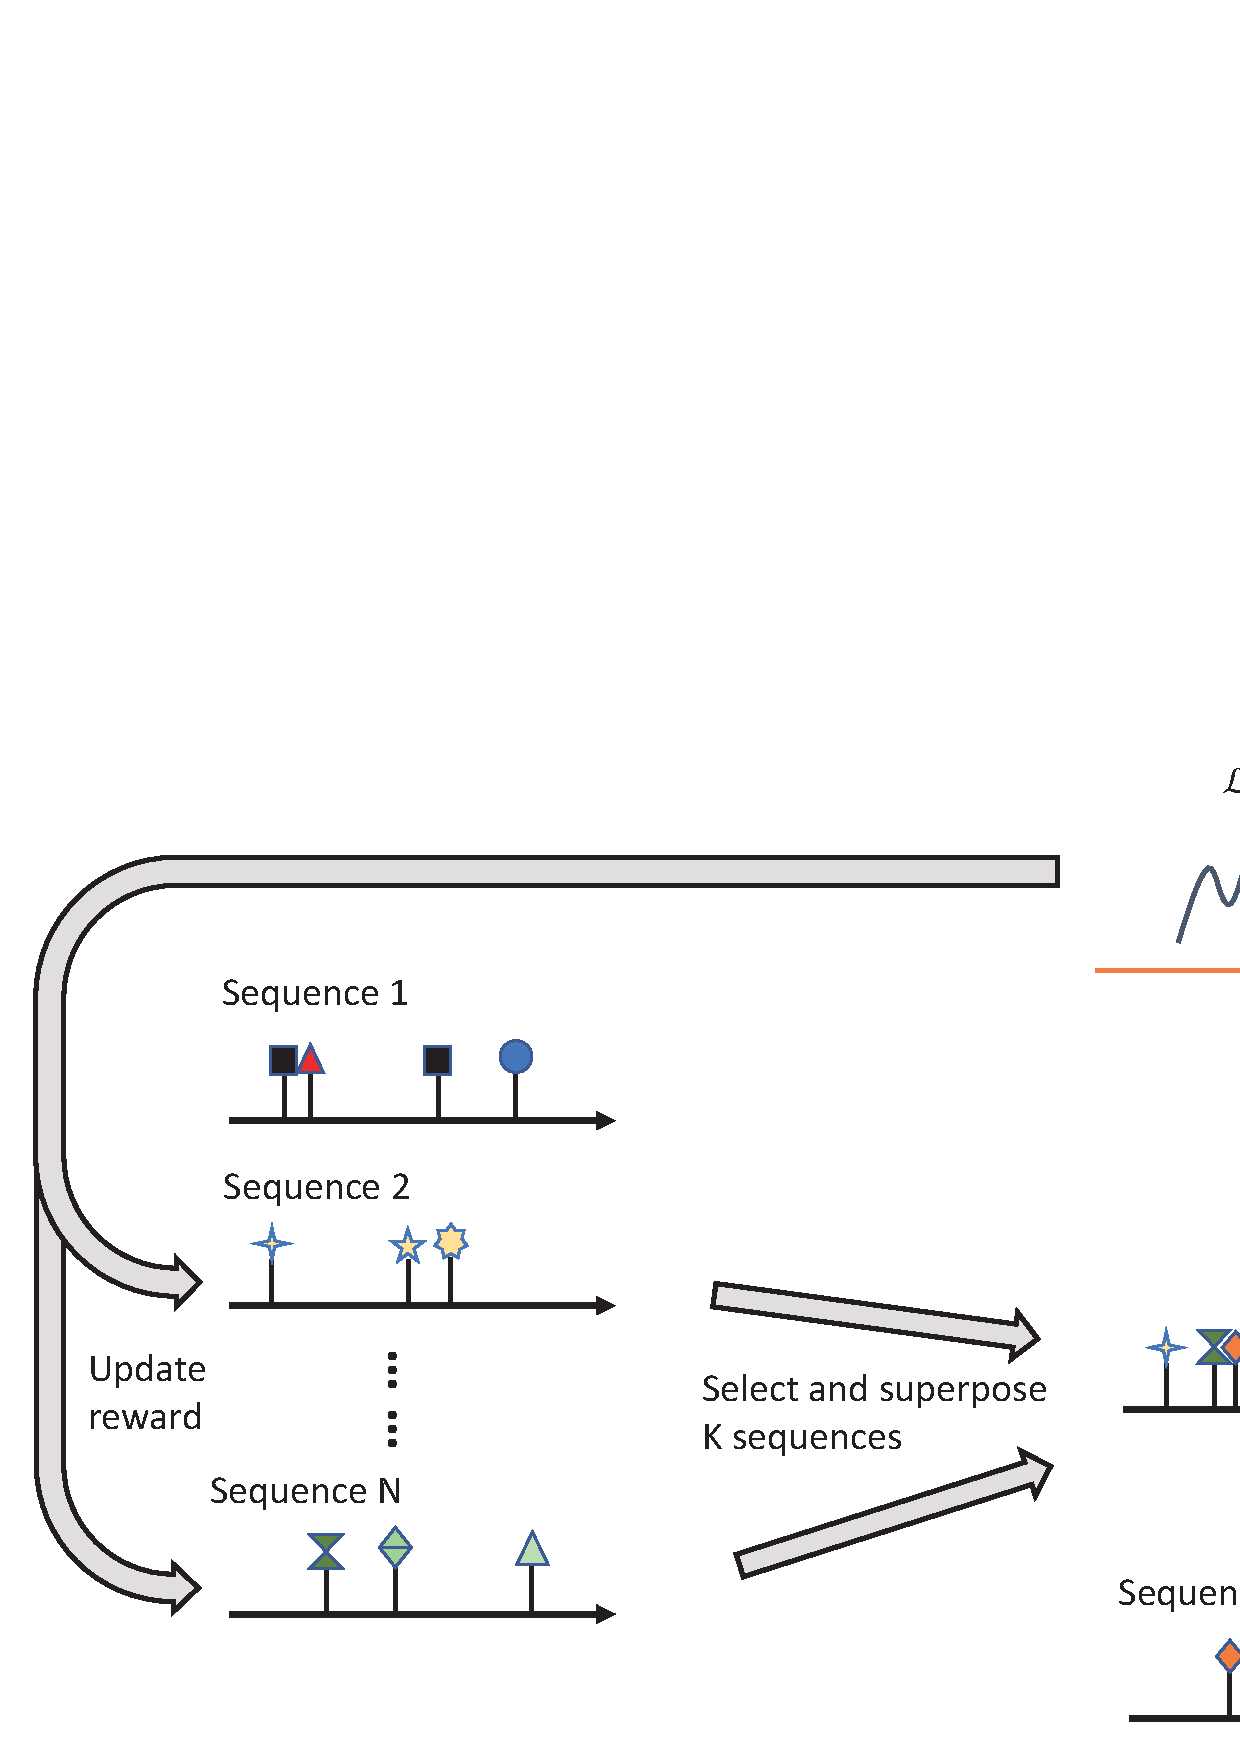
\includegraphics[width=0.6\linewidth]{figure1.png}}
\label{fig1}
\caption{The overall framework of the proposed method.}
\end{figure}


\end{frame}


\begin{frame}{Notation}
\begin{itemize}
    \item $G=(A,X)$, a labeled graph for a molecule, where $A \in \{0,1\}^{n \times n \times b}$ is the adjacency matrix and $X \in \{0,1\}^{n \times d}$ the matrix of node features;
    \item $n$, the number of atoms; 
    \item $b$, the number of bond types;
    \item $d$, the dimension of node features;
    \item $(\{G_i\}_{i=1}^{N_1},G_p)$, a reaction where $G_i$ denotes a reactant graph and $G_p$ a product graph
\end{itemize}
\end{frame}







\begin{frame}[noframenumbering]

\begin{itemize}

    \begin{LARGE}
    
    \item \light{Introduction}
    
    \item Reaction Center Identification
    
    \item \light{Reactants Generation via Variational Graph Translation}

    \end{LARGE}
    
\end{itemize}
	
\end{frame}







\begin{frame}{Reaction Center}

Reaction center means an atom pair $(i, j)$ that satisfies:

\begin{itemize}
    \item there is a bond between the $i$-th and $j$-th nodes in the \textbf{product} graph;
    \item there is \textbf{no} bond between the $i$-th and $j$-th nodes in the
\textbf{reactant} graph.
\end{itemize}

\pause

Synthons are subgraphs extracted from the products by breaking the bonds in the reaction centers.
    
\end{frame}









\begin{frame}{Reaction Center Identification}

The reactivity score of the atom pair $(i, j)$ is calculated as:

\begin{eqnarray}
\begin{aligned}
s_{ij} = \sigma(m_r(e_{ij}))
\end{aligned}    
\end{eqnarray}

where $m_r$ is a feedforward network that maps $e_{ij}$ to a scalar, $\sigma(\cdot)$ denotes the Sigmoid function, and $e_{ij}$ the edge embedding.

\pause

\begin{eqnarray}
\begin{aligned}
\mathcal{L}_1 = - \sum_r \sum_{i \ne j} \lambda Y_{ij} \log(s_{ij}) + (1-Y_{ij})\log(1-s_{ij})
\end{aligned}    
\end{eqnarray}

where $Y \in \{0,1\}^{n \times n}$ indicates the reaction centers.

\end{frame}









\begin{frame}{The Edge Embedding}

\begin{eqnarray}
\begin{aligned}
e_{ij} = H_i^L \ \| \ H_j^L \ \| \ A_{ij} \ \| \ h_{G_p}
\end{aligned}    
\end{eqnarray}

where $H^L \in \mathbb{R}^{n \times k}$ denotes the node embeddings, and $h_{G_p}$ denotes the entire graph embedding of product $G_p$.




\end{frame}








\begin{frame}{The Node Embedding}

R-GCN, a variant of Relational GCN,

\begin{eqnarray}
\begin{aligned}
H^L = \text{R-GCN}(G_p)
\end{aligned}    
\end{eqnarray}

For the $l$-th layer,

\begin{eqnarray}
\begin{aligned}
H^l = \text{Agg} (\text{ReLu} ( \{E_i H^{l-1} W_i^l\} | i \in (1, \ldots, b)))
\end{aligned}    
\end{eqnarray}

where $E_i = A_{[:,:,i]} + I$ denotes the adjacency matrix of the $i$-th edge type, $W_i^l$ is the trainable weight matrix for the $i$-th edge type, and $\text{Agg} (\cdot)$ denotes an aggregation function.



\end{frame}








\begin{frame}[noframenumbering]

\begin{itemize}

    \begin{LARGE}
    
    \item \light{Introduction}
    
    \item \light{Reaction Center Identification}
    
    \item Reactants Generation via Variational Graph Translation

    \end{LARGE}
    
\end{itemize}
	
\end{frame}







\begin{frame}{Reactants Generation via Variational Graph Translation}

\begin{eqnarray*}
\begin{aligned}
(\{G_i\}_{i=1}^{N_1}, G_p) \to (\{G_i\}_{i=1}^{N_1}, \{S_i\}_{i=1}^{N_1})
\end{aligned}    
\end{eqnarray*}

\pause

\begin{eqnarray*}
\begin{aligned}
p(G|S)
\end{aligned}    
\end{eqnarray*}

\pause

\begin{eqnarray*}
\begin{aligned}
p(G|z, S)
\end{aligned}    
\end{eqnarray*}

where $z$ denotes a low-dimensional latent vector.


\end{frame}









\begin{frame}{The Generative Model}

Let $t=(a_1,\ldots,a_T) \in \mathcal{T}$ be a sequence of graph transformation actions, and $\mathcal{T}$ be the collection of all trajectories that can translate synthons $S$ to target reactants $G$,

\begin{eqnarray*}
\begin{aligned}
P(G|z, S) \to  P(t|z, S)
\end{aligned}    
\end{eqnarray*}


\end{frame}





\begin{frame}{The Generative Model}


Let $S^i$ denote the graph after applying the sequence of actions $a_{1:i}$ to $S$,

\begin{eqnarray*}
\begin{aligned}
P(S^i|S^{i-1},z) = P(a_i|S^{i-1},z)
\end{aligned}    
\end{eqnarray*}

\pause

Use the assumption of a Markov Decision Process (MDP),

\begin{eqnarray}
\begin{aligned}
p(t|z,S) = p(a_{1:T}|z, S) = \prod_{i=1}^{T} p(a_i|S^{i-1}, z)
\end{aligned}    
\end{eqnarray}

\end{frame}








\begin{frame}{The Defination of an Action}

\begin{eqnarray}
\begin{aligned}
a_i = (a_i^1,a_i^2,a_i^3,a_i^4)
\end{aligned}    
\end{eqnarray}

\begin{itemize}
    \item $a_i^1 \in \{0, 1\}^2$ predicts the termination of the graph translation procedure;
    \item $a_i^2 \in \{0, 1\}^n$ indicates the first node;
    \item $a_i^3 \in \{0, 1\}^{n+m}$ indicates the second node;
    \item $a_i^4 \in \{0, 1\}^{b}$ predicts the bond type between two nodes.
\end{itemize}


\end{frame}





\begin{frame}{Termination Prediction}

\begin{eqnarray*}
\begin{aligned}
&H = \mathcal{R}(S^{i-1}),\ h_S = \text{Readout}(H) \\
&p(a_i^1|z, S^{i-1})=\tau(m_t(h_S, z))
\end{aligned}    
\end{eqnarray*}

where $\tau(\cdot)$ denotes the softmax function, and $m_t(\cdot)$ is a feedforward network.

\end{frame}







\begin{frame}{Nodes Selection}

\begin{eqnarray*}
\begin{aligned}
&p(a_i^2|z,S^{i-1},a_i^1)=\tau(\beta_1 \odot m_f(\mathcal{R}(\tilde{S}^{i-1}), z))\\
&a_i^2 \sim p(a_i^2|z,S^{i-1},a_i^1)\\
&p(a_i^3|z,S^{i-1},a_i^{1:2})=\tau(\beta_2 \odot m_s(\mathcal{R}(\tilde{S}^{i-1}), z,a_i^2))\\
&a_i^3 \sim p(a_i^3|z,S^{i-1},a_i^{1:2})\\
\end{aligned}    
\end{eqnarray*}

where $\tilde{S}^{i-1} = S^{i-1} \cup V$, $V$ is the set of possible atoms to be added during graph translation. $m_f(\cdot)$ and $m_s(\cdot)$ are feedforward networks. $\beta_1$ and $\beta_2$ are masks to zero out the probability of certain atoms
being selected.

\end{frame}






\begin{frame}{Edge Labeling}

\begin{eqnarray*}
\begin{aligned}
&p(a_i^4|z,S^{i-1},a_i^{1:3})=\tau(m_e(\mathcal{R}(\tilde{S}^{i-1}), z, a_i^{2:3}))\\
&a_i^4 \sim p(a_i^4|z,S^{i-1},a_i^{1:3})
\end{aligned}    
\end{eqnarray*}

where $m_e(\cdot)$ is a feedforward networks.

\end{frame}






\begin{frame}{Reactants Generation via Variational Graph Translation}

\begin{figure}[t]
\centerline{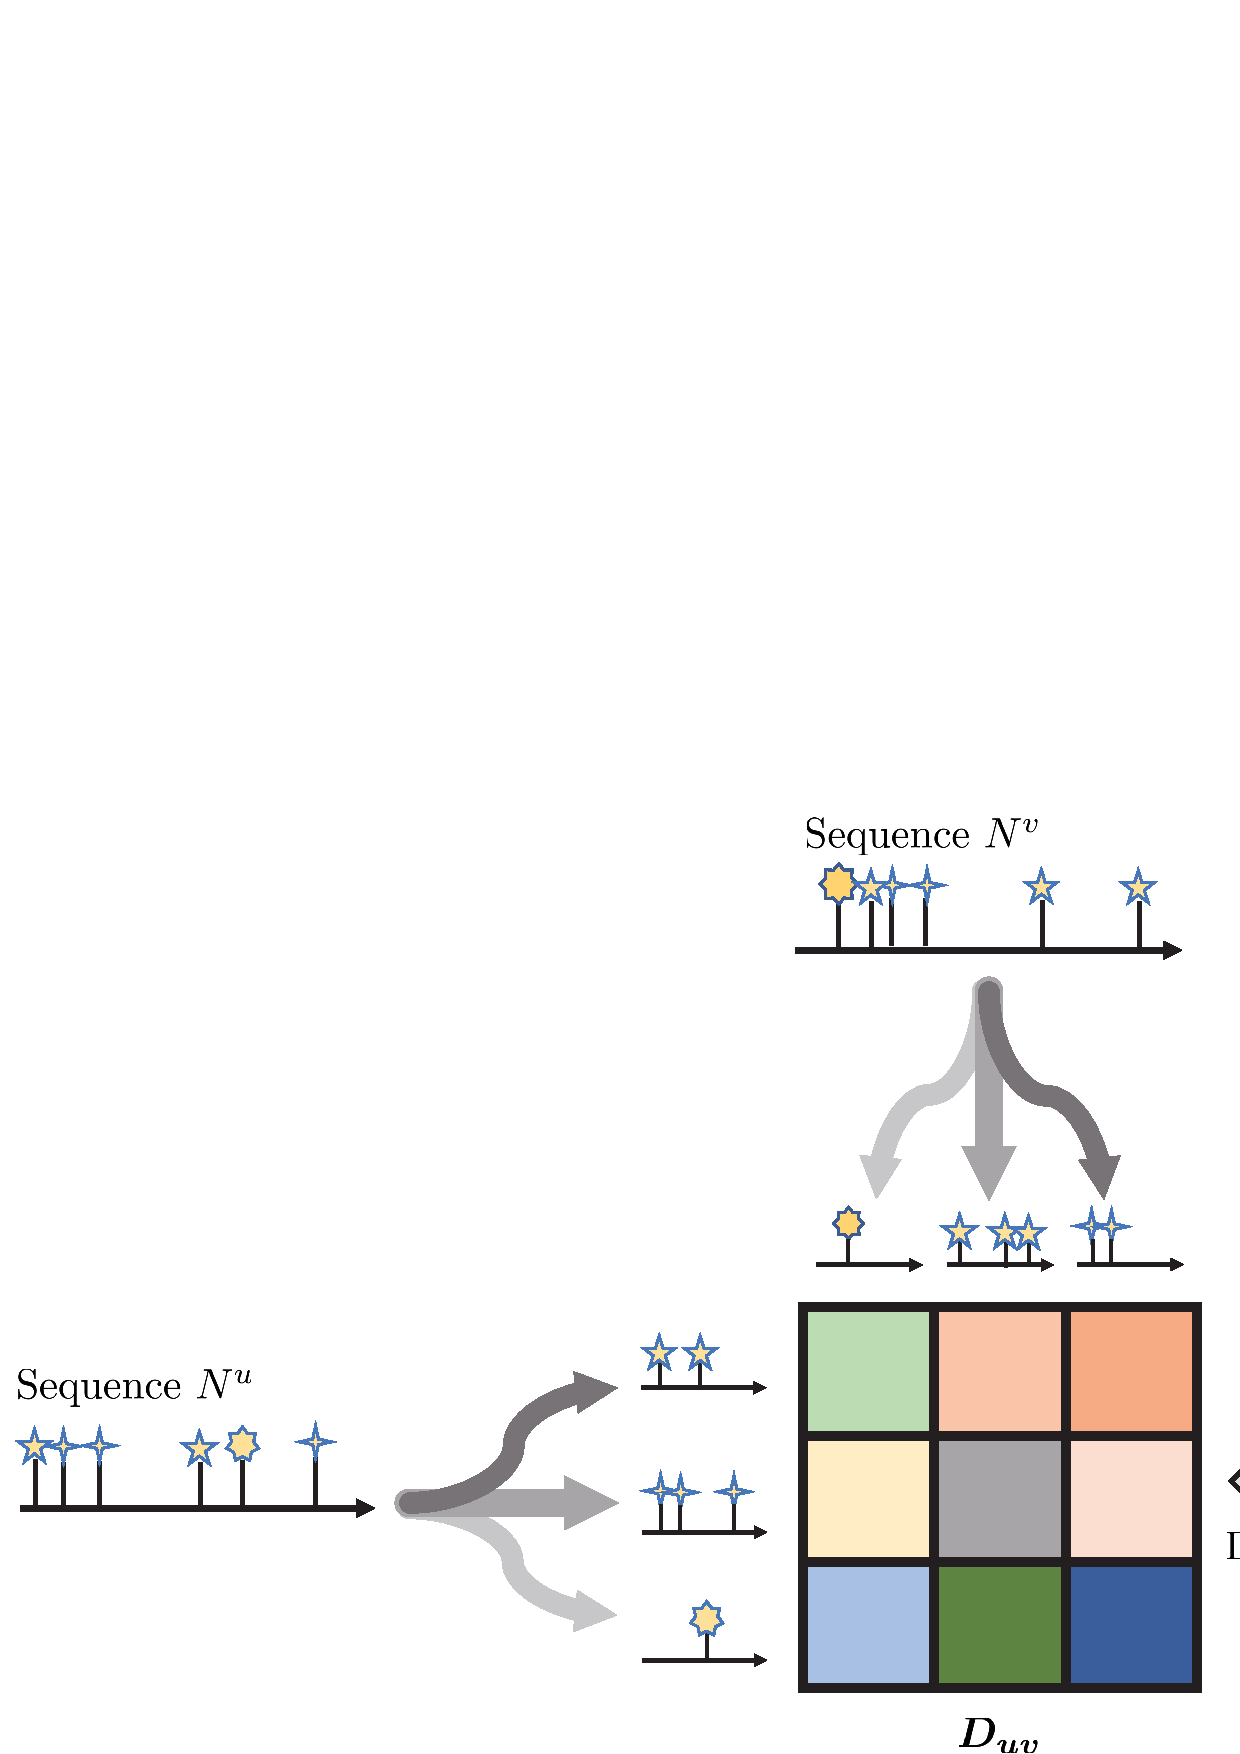
\includegraphics[width=1.0\linewidth]{figure2.png}}
\label{fig2}
\caption{Illustration of the proposed variational graph translation module.}
\end{figure}

\end{frame}


\end{document}	% Done!

